% Briefly comment on your design specifications, assumptions,
% shortcomings, and included extra features (if any). Highlight any
% differences between your design and stated specifications. Summarize
% lessons learned while doing the lab and provide advice.

\section{Discussion}
\subsection{Limiting Factors}
The largest factors in the design was that of simplicity and clearness
over optimization and performance. As the time constraint was the
dominant factor in this lab, decisions tended to be in favour of that
which complimented the limited amount of time available.

\subsubsection{Software Factors}
Software factors in the design include the use of \gls{spi} to greatly
simplify the \gls{lcd} interface and an abstracted hardware interface to
allow faster development. Using \gls{spi} reduced wiring and \gls{gpio}
port setup and avoided potential "bit banging", or sending a series of
hard-coded bits reducing flexibility of development and coordination of
parallelizing serialized data. \\

\subsubsection{Hardware Factors}
Hardware design factors consisted of ensuring the measured frequency from the \gls{pwm} signal generator was within the range of 0 to 9999, so that all decimal figures can fit on the \gls{lcd} display. To do this, R1, R2, and C1 from Figure \ref{fig:555} were selected as \SI{1}{\kilo \ohm}, \SI{4.7}{\kilo \ohm}, and \SI{470}{\nano \farad} respectively. The supply voltage was \SI{5}{\volt}. Using the equation f = $\frac{1.443}{(R1 + 2R2)C1}, the frequency when the optocoupler is off is $\sim 295\si{\hertz}.

By measuring the resistance between the collector and emitter of the optocoupler transistor when the \gls{dac} is supplying $\sim 3.3\si{\volts}, this 

\begin{figure}
	\caption{555 Timer Configuration}
	\centering
	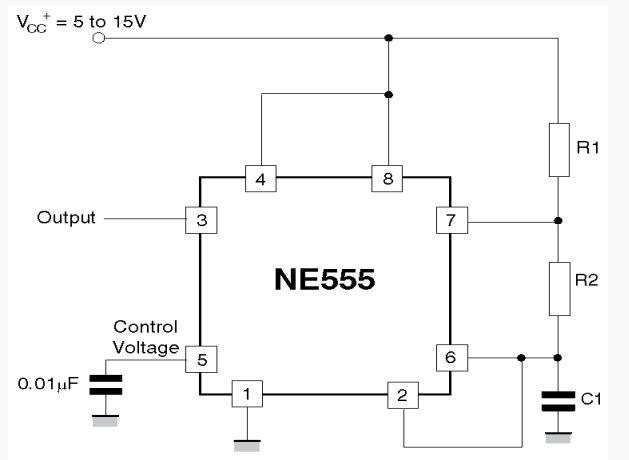
\includegraphics[scale=0.5]{figures/555-timer}
	\label{fig:555}
\end{figure}
\begin{figure}
	\caption{System Interfacing Diagram}
	\centering
	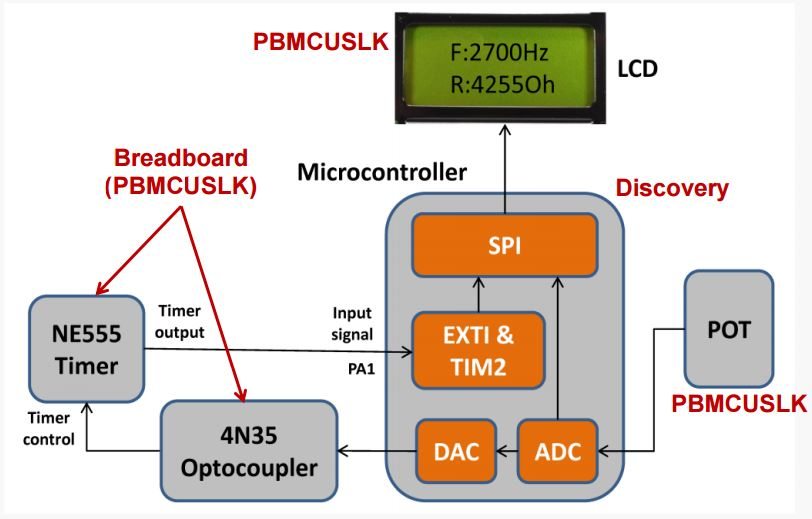
\includegraphics[scale=0.5]{figures/system-diagram}
	\label{fig:system}
\end{figure}

\subsubsection{Effects}
The simple design of the \gls{pwm} signal generator lead to a small
range of producible frequencies with a relatively low resolution. A more
complicated design may have been able to produce a wider range with more
coverage. The trade-off for simplicity over optimization also resulted
in a slower response time than could be achieved with a more complex
design. Placing the \gls{lcd} update code in the frequency monitor
interrupt lead to simplicity with the \gls{lcd} only changing when there
was an update and avoided interrupts being serviced while writing to the
\gls{lcd}, however this also decreased the maximum update rate of the
frequency monitor. This was deemed to be an acceptable trade-off as the
measured frequency wasn't being supplied to another component other than
the \gls{lcd} for human observation and thus the maximum speed
observable was deemed the maximum necessary speed of measurement.
